

\tikzset{every picture/.style={line width=0.75pt}} %set default line width to 0.75pt        

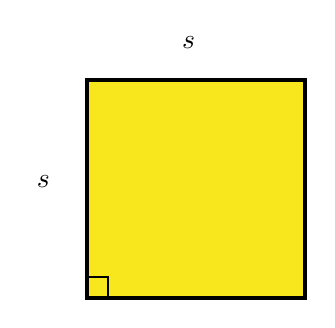
\begin{tikzpicture}[x=0.75pt,y=0.75pt,yscale=-1,xscale=1]
%uncomment if require: \path (0,167); %set diagram left start at 0, and has height of 167

%Shape: Square [id:dp9958510811050907] 
\draw  [fill={rgb, 255:red, 248; green, 231; blue, 28 }  ,fill opacity=1 ][line width=1.5]  (207,37) -- (312,37) -- (312,142) -- (207,142) -- cycle ;
%Shape: Square [id:dp2209502611968972] 
\draw   (207,132) -- (217,132) -- (217,142) -- (207,142) -- cycle ;

% Text Node
\draw (186,86) node   {$s$};
% Text Node
\draw (256,19) node   {$s$};
% Text Node
% \draw (411,87) node   {$ \begin{array}{l}
% \boldsymbol{A\ =\ s^{2}}\\
% \\
% \boldsymbol{P\ =\ 4s}
% \end{array}$};


\end{tikzpicture}